% Bản tiếng Việt để đọc nội bộ (không nộp) của bài Track 2. Biên dịch: xelatex main_vi; bibtex main_vi; xelatex main_vi x2.
% Luật viết: skill upar-paper-rules. Thuật ngữ theo PLAN.md. Số liệu: analysis/*.json và analysis/knn_logs_2026-10-11.txt.
\documentclass[10pt,twocolumn,letterpaper]{article}

\usepackage[review,algorithms]{wacv}
\usepackage{fontspec}
\setmainfont{Liberation Serif}
\setsansfont{Liberation Sans}

%
% --- inline annotations
%
\newcommand{\red}[1]{{\color{red}#1}}
\newcommand{\todo}[1]{{\color{red}#1}}
\newcommand{\TODO}[1]{\textbf{\color{red}[TODO: #1]}}
% --- disable by uncommenting  
% \renewcommand{\TODO}[1]{}
% \renewcommand{\todo}[1]{#1}


\usepackage{booktabs}
\usepackage{amsmath}
\usepackage{graphicx}
\graphicspath{{figs/}}

\definecolor{wacvblue}{rgb}{0.21,0.49,0.74}
\usepackage[pagebackref,breaklinks,colorlinks,allcolors=wacvblue]{hyperref}
\usepackage[capitalize]{cleveref}
% wacv.sty sets the cleveref names at the end of the preamble, so the Vietnamese names go in \AtBeginDocument
\AtBeginDocument{%
\crefname{section}{Mục}{Mục}\Crefname{section}{Mục}{Mục}%
\crefname{subsection}{Mục}{Mục}\Crefname{subsection}{Mục}{Mục}%
\crefname{figure}{Hình}{Hình}\Crefname{figure}{Hình}{Hình}%
\crefname{table}{Bảng}{Bảng}\Crefname{table}{Bảng}{Bảng}%
\crefname{equation}{Pt.}{Pt.}\Crefname{equation}{Pt.}{Pt.}%
\renewcommand{\crefpairconjunction}{ và }%
\renewcommand{\crefmiddleconjunction}{, }%
\renewcommand{\creflastconjunction}{ và }%
}
\renewcommand{\figurename}{Hình}
\renewcommand{\tablename}{Bảng}
\renewcommand{\refname}{Tài liệu tham khảo}
\def\elvbf{\fontsize{11}{13}\selectfont\bfseries}\def\tenbf{\fontsize{10}{12}\selectfont\bfseries}
\def\abstract{\centerline{\large\bf Tóm tắt}\vspace*{12pt}\noindent\it\ignorespaces}

\def\wacvPaperID{*****}
\def\confName{WACV}
\def\confYear{2027}

\title{Xếp hạng theo likelihood, làm mượt theo láng giềng:\\dùng foundation encoder cho truy xuất người theo thuộc tính\\trên camera chưa từng thấy}
\author{Bản tiếng Việt để đọc nội bộ (không nộp)}

\begin{document}
\maketitle

%=====================================================================
\begin{abstract}
Bài báo này trình bày giải pháp của nhóm cho Track~2, truy xuất người theo thuộc tính, của UPAR Challenge 2027 tại workshop Real-World Surveillance của WACV 2027. Truy xuất người theo thuộc tính tìm một người trong ảnh camera giám sát chỉ từ một mô tả như giới tính, độ tuổi, màu quần áo và phụ kiện, không cần ảnh mẫu của người đó. Bài toán khó khi ảnh đến từ những camera không có trong dữ liệu train, vì xác suất thuộc tính mà mô hình dự đoán bị lệch trên camera mới. Phương pháp thường dùng xếp hạng ảnh theo khoảng cách L1 giữa xác suất thuộc tính dự đoán và truy vấn, và ở hai mùa trước không đội nào vượt được baseline của ban tổ chức ở track này. Nhóm dùng hai foundation encoder là DINOv3 và CLIP, fine-tune riêng, và thay đổi ba chỗ. Mỗi ảnh được chấm bằng log-likelihood của đúng truy vấn thay cho khoảng cách L1. Mô hình được train thêm một cross-entropy cho các nhóm thuộc tính loại trừ nhau, như các khoảng tuổi hay các màu áo. Logit của mỗi ảnh được làm mượt với logit của các láng giềng gần của nó trong gallery, tìm theo đặc trưng của DINOv3. Trong các thí nghiệm leave-one-dataset-out, cả ba thay đổi đều nâng mADM trên cả hai held-out dataset, và riêng điểm likelihood nâng cả sáu độ đo truy xuất. Bước làm mượt không cần train, và khi dùng đặc trưng DINOv3 chưa fine-tune, nó nâng mADM ở mọi mô hình nhóm đã thử. Ngược lại, hiệu chỉnh xác suất sau khi train bằng dữ liệu của các dataset nguồn làm mADM giảm. Trên tập test ẩn của cuộc thi, hệ thống đạt mADM 0.6817.
\end{abstract}

\begin{figure*}[t]
\centering
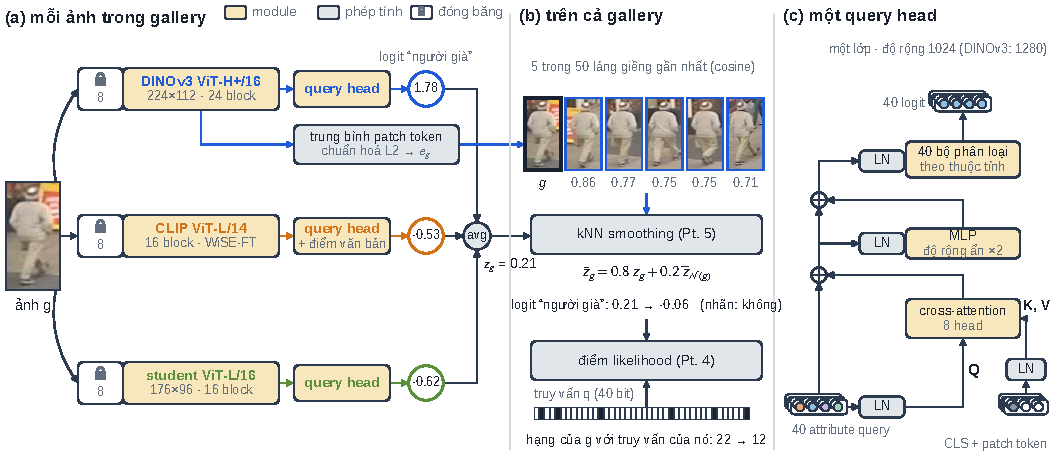
\includegraphics[width=\linewidth]{arch_vi.pdf}
\caption{(a) Ba mô hình chạy trên một ảnh $g$ của gallery PETA. Mỗi encoder đóng băng patch embedding và tám block đầu (khối có ổ khoá) và fine-tune các block còn lại cùng một query head. Các hình tròn là logit của thuộc tính tuổi già (Age-Old) của ba mô hình thuộc fold giữ ngoài PETA, nên chúng chưa thấy ảnh PETA nào khi train, và trung bình của ba logit là $z_g$. Trong cùng lượt chạy, trung bình các patch token của DINOv3 ViT-H+/16 sau khi chuẩn hoá L2 là đặc trưng ngoại hình $e_g$. (b) Năm trong 50 láng giềng gần nhất của $g$ theo cosine giữa các $e_g$, đều là cùng một người ở các khung hình khác. Láng giềng trong hình được tìm bằng mô hình DINOv3 đã nộp, và mô hình này đã thấy các ảnh validation này khi train. Sau kNN smoothing (\cref{eq:knn}), logit tuổi già đổi dấu về đúng nhãn. Với truy vấn tạo từ chính nhãn của $g$, hạng của $g$ trong gallery theo điểm likelihood (\cref{eq:ll}) tăng từ 22 lên 12. (c) Một query head. Ba mô hình có cùng thiết kế query head, và query head của CLIP cộng thêm một điểm văn bản.}
\label{fig:arch}
\end{figure*}

%=====================================================================
\section{Giới thiệu}
\label{sec:intro}

Truy xuất người theo thuộc tính cho phép tìm một người trong ảnh camera giám sát chỉ từ một mô tả bằng lời, như giới tính, độ tuổi, màu quần áo và phụ kiện, mà không cần ảnh mẫu của người đó~\cite{upar}. Bài toán thường được giải bằng cách nhận dạng thuộc tính cho từng ảnh rồi so các dự đoán với truy vấn~\cite{upar,specker21}. Một khó khăn lớn xuất hiện khi ảnh đến từ camera chưa từng thấy. Độ phân giải, góc camera và ánh sáng thay đổi giữa các camera, và mỗi dataset train gán nhãn theo quy tắc riêng. Vì vậy xác suất thuộc tính khớp tốt với camera train có thể lệch trên camera mới, và thứ hạng tạo từ các xác suất đó cũng lệch theo.

Bài báo này trình bày giải pháp của nhóm cho Track~2 của UPAR Challenge 2027, tổ chức tại workshop Real-World Surveillance (RWS) của WACV 2027 và tiếp nối các mùa 2023 và 2024~\cite{upar23,upar24}. Mô hình được train trên PA100k~\cite{pa100k}, PETA~\cite{peta} và Market-1501~\cite{market,marketattr}, rồi được test trên ảnh của những camera khác. Ở hai mùa trước, không đội nào vượt được baseline của ban tổ chức ở track truy xuất, dù nhiều đội đã vượt baseline ở track nhận dạng thuộc tính~\cite{upar23,upar24}. Báo cáo năm 2024 cho rằng mô hình trở nên quá tự tin hoặc thiếu tự tin trên camera mới, và các xác suất lệch này làm sai lệch khoảng cách tới truy vấn~\cite{upar24}. Code mẫu của cuộc thi năm nay vẫn xếp hạng theo khoảng cách L1~\cite{starterkit}.

Nhóm dùng hai foundation encoder có cách pretrain khác nhau là DINOv3~\cite{dinov3} và CLIP~\cite{clip}, mỗi encoder được fine-tune riêng với một query head~\cite{q2l}, và lấy trung bình logit của chúng cùng một student được distill từ hai teacher~\cite{hinton,patient} (\cref{fig:arch}). Hệ thống thay đổi ba chỗ trong cách biến dự đoán thành thứ hạng. Thứ nhất, mỗi ảnh được chấm bằng log-likelihood của đúng truy vấn thay cho khoảng cách L1, tương tự cách DAP chấm một lớp từ các thuộc tính~\cite{dap}. Thứ hai, điểm này coi các thuộc tính độc lập, trong khi nhiều nhóm thuộc tính loại trừ nhau, nên mô hình được train thêm một cross-entropy cho từng nhóm như vậy. Thứ ba, logit của mỗi ảnh được trộn với logit của các láng giềng gần của nó trong gallery, tìm theo đặc trưng ngoại hình từ chính lượt chạy của DINOv3. Bước này giống database-side augmentation trong truy xuất ảnh~\cite{turcot,gordo}, và luật của Track~2 cho phép re-ranking tự động như vậy, miễn là không khai thác thông tin riêng nào về tập test ẩn~\cite{rules}.

Mọi lựa chọn được đánh giá trên một dataset không có trong dữ liệu train và với cùng các mô hình đã train, nên chênh lệch chỉ đến từ bước đang được kiểm tra. Hai kết luận về cách chấm điểm và về hiệu chỉnh xác suất còn được kiểm tra lại trên các mô hình của giai đoạn phát triển, và hệ thống được kiểm tra trên tập test ẩn. Các đóng góp chính của bài như sau.
\begin{itemize}
\item Chấm điểm bằng log-likelihood của đúng truy vấn tốt hơn khoảng cách L1 ở mọi độ đo truy xuất, trên cả hai held-out dataset và trên mọi mô hình của giai đoạn phát triển. Khoảng cách L1 xếp một ảnh sai đúng một thuộc tính với độ tin cao lên trước ảnh khớp đúng có nhiều thuộc tính hơi không chắc chắn.
\item Sai lệch calibration là có thật nhưng không sửa được sau khi train. Hiệu chỉnh khớp trên nhãn của held-out dataset sẽ nâng mADM, nhưng hiệu chỉnh khớp trên các dataset nguồn lại làm mADM giảm. Lượng sai lệch trên dữ liệu nguồn cùng cỡ với trên held-out dataset, nhưng hướng sai lệch của từng thuộc tính khác nhau giữa hai nơi.
\item Cross-entropy cho các nhóm thuộc tính loại trừ nhau nâng mADM trên cả hai held-out dataset, cả khi dùng riêng lẫn khi dùng cùng kNN smoothing.
\item kNN smoothing không cần train và không phụ thuộc mô hình nhận dạng. Với đặc trưng của DINOv3 chưa fine-tune, nó nâng mADM ở mọi mô hình của giai đoạn phát triển trên cả hai held-out dataset, và phần tăng đến từ đặc trưng ngoại hình chứ không đến từ việc lấy trung bình bất kỳ.
\end{itemize}

%=====================================================================
\section{Công trình liên quan}
\label{sec:related}

\paragraph{Truy xuất người theo thuộc tính.} Các phương pháp truy xuất người theo thuộc tính hoặc nhận dạng thuộc tính rồi so dự đoán với truy vấn, hoặc học một không gian chung cho mô tả thuộc tính và ảnh~\cite{upar}. Cách thứ nhất cho kết quả dễ giải thích, vì mỗi thành phần của điểm ứng với một thuộc tính~\cite{upar}. Với cách này, việc gộp điểm của nhiều bộ phân loại thuộc tính đã được nghiên cứu từ trước. Siddiquie \etal xếp hạng ảnh cho truy vấn nhiều thuộc tính và mô hình hoá tương quan giữa các thuộc tính~\cite{siddiquie}. Scheirer \etal biến điểm thô của từng bộ phân loại thành xác suất trước khi gộp, và bước chuẩn hoá này không cần nhãn~\cite{scheirer}. DAP chấm một lớp bằng tích các xác suất thuộc tính của lớp đó, chia cho xác suất tiên nghiệm của chúng~\cite{dap}. Điểm likelihood của nhóm có cùng dạng tích nhưng không chia cho xác suất tiên nghiệm. Với UPAR, Specker và Beyerer chỉ ra rằng các phương pháp khi đó dùng khoảng cách Euclid giữa truy vấn và dự đoán. Họ đề xuất một khoảng cách tính đến phân phối đầu ra của bộ phân loại, kèm hiệu chỉnh xác suất và trọng số theo sai số dự đoán của từng thuộc tính~\cite{specker21}. Sau đó họ đề xuất một mô hình nhận dạng tốt cả cho từng thuộc tính lẫn cho truy xuất, cùng độ đo mADM~\cite{specker23}. Baseline của cuộc thi gồm ConvNeXt và một lớp fully-connected, train bằng weighted cross-entropy~\cite{upar23}. Công trình gần nhất với bài này là~\cite{specker21}, vì nó cũng thay khoảng cách và hiệu chỉnh xác suất. Bài này dùng xác suất khớp đúng thay cho một khoảng cách, và đo trực tiếp xem hiệu chỉnh học trên dữ liệu nguồn có còn đúng trên dataset không có trong dữ liệu train hay không.

\paragraph{Calibration khi dữ liệu dịch chuyển.} Hiệu chỉnh xác suất biến điểm của bộ phân loại thành xác suất bằng một hàm nhỏ khớp trên dữ liệu có nhãn. Platt scaling khớp một hàm sigmoid lên điểm này~\cite{platt}. Temperature scaling dùng chung một hệ số cho mọi lớp và giảm được phần lớn sai lệch calibration của mạng nơ-ron trên dữ liệu cùng phân phối~\cite{guo}. Cả hai cách đều cần dữ liệu có nhãn từ cùng phân phối với dữ liệu test. Ovadia \etal cho thấy calibration của các mô hình học sâu kém đi khi dữ liệu dịch chuyển, kể cả sau temperature scaling~\cite{ovadia}. Kull và Flach tách một hàm loss đúng đắn (proper scoring rule) thành nhiều phần, trong đó thành phần calibration là phần mà một hàm hiệu chỉnh tối ưu loại bỏ được~\cite{kull}. Nhóm dùng thành phần này để so sai lệch calibration của cùng một mô hình trên dữ liệu nguồn và trên held-out dataset.

\paragraph{Tận dụng gallery khi xếp hạng.} Ngoài việc sửa riêng từng dự đoán, thứ hạng còn có thể dùng các ảnh khác trong gallery. Trong re-identification, k-reciprocal re-ranking dùng quan hệ láng giềng giữa truy vấn và các ảnh gallery để xếp hạng lại~\cite{kreciprocal}. Trong truy xuất ảnh, query expansion dùng các kết quả đầu để tạo truy vấn mới~\cite{chum07}. Database-side augmentation thay biểu diễn của mỗi ảnh trong cơ sở dữ liệu bằng một tổ hợp của chính nó và các láng giềng~\cite{turcot,arandjelovic,gordo}. Các cách này so truy vấn và gallery trong cùng một không gian đặc trưng. Trong truy xuất theo thuộc tính, truy vấn là một vector nhị phân và không có ảnh. Vì vậy nhóm áp dụng ý tưởng database-side augmentation cho logit thuộc tính của gallery, còn láng giềng được tìm trong không gian đặc trưng ảnh. LAME~\cite{lame} cũng điều chỉnh đầu ra của mô hình theo đồ thị láng giềng của các mẫu test. LAME giải một bài toán tối ưu cho phân loại, còn kNN smoothing của nhóm chỉ là một bước lấy trung bình có trọng số cố định.

\paragraph{Foundation encoder và ensemble.} Logit mà kNN smoothing lấy trung bình đến từ hai foundation encoder đã fine-tune là DINOv3~\cite{dinov3} và CLIP~\cite{clip}, với cách pretrain khác nhau. Fine-tune có thể làm suy giảm đặc trưng đã pretrain và làm giảm độ chính xác khi phân phối dữ liệu thay đổi~\cite{lpft}. WiSE-FT giảm hiện tượng này bằng cách nội suy giữa trọng số pretrain và trọng số đã fine-tune~\cite{wiseft}. Lấy trung bình dự đoán của nhiều mô hình, mỗi mô hình được train riêng, cho dự đoán chính xác hơn và xác suất đáng tin hơn so với từng mô hình~\cite{deepens}. Distillation chuyển dự đoán của các teacher sang một student~\cite{hinton}, và hiệu quả hơn khi teacher và student cùng thấy một ảnh đã biến đổi và được train đủ lâu~\cite{patient}. Bài này dùng các thành phần đã biết đó để có xác suất thuộc tính tốt, và tập trung vào bước biến xác suất thành thứ hạng.

%=====================================================================
\section{Phương pháp}
\label{sec:method}

Hệ thống nhận một truy vấn gồm 40 thuộc tính nhị phân và một gallery ảnh người đã cắt, rồi trả về thứ hạng của toàn bộ gallery (\cref{fig:arch}). Ba mô hình nhận dạng thuộc tính chạy trên mỗi ảnh, và trung bình logit của chúng được làm mượt theo các ảnh giống nó trong gallery. Mỗi ảnh sau đó được chấm bằng log-likelihood của truy vấn, và gallery được xếp theo điểm này.

\paragraph{Bài toán và độ đo.} Gallery là một tập ảnh người đã được cắt sẵn. Mỗi truy vấn là một vector $q\in\{0,1\}^{K}$ với $K=40$ thuộc tính. Cuộc thi tạo một truy vấn cho mỗi vector nhãn khác nhau trong gallery, và một ảnh khớp đúng với truy vấn khi cả 40 nhãn của ảnh bằng truy vấn. Với mỗi truy vấn, hệ thống trả về thứ hạng của toàn bộ gallery. Độ đo chính là mADM~\cite{specker23}. Gọi $\mathrm{dom}(q,g)$ là tỷ lệ thuộc tính mà ảnh $g$ khớp với $q$. Độ khớp được chuẩn hoá theo từng truy vấn
\begin{equation}
\mathrm{ndom}(q,g)=\max\Big(0,\frac{\mathrm{dom}(q,g)-\overline{\mathrm{dom}}_q}{\max_{g'}\mathrm{dom}(q,g')-\overline{\mathrm{dom}}_q}\Big),
\label{eq:ndom}
\end{equation}
trong đó $\overline{\mathrm{dom}}_q$ là trung bình trên gallery. Gọi $r_1<\dots<r_R$ là hạng của $R$ ảnh khớp đúng và $g_{(j)}$ là ảnh ở hạng $j$. Khi đó
\begin{equation}
\mathrm{ADM}(q)=\frac1R\sum_{m=1}^{R}\frac{1}{r_m}\sum_{j\le r_m}\mathrm{ndom}\big(q,g_{(j)}\big),
\label{eq:adm}
\end{equation}
và mADM là trung bình của ADM trên các truy vấn. ADM giống average precision, nhưng mỗi ảnh đứng trước một ảnh khớp đúng được tính điểm bằng độ khớp của nó thay vì 0 hoặc 1. Vì vậy các ảnh khớp đúng quyết định vị trí lấy điểm, còn các ảnh gần khớp đứng trước chúng vẫn được một phần điểm. Nhóm cũng báo cáo mAP, mINP và Rank-1, Rank-5, Rank-10 như leaderboard. Mọi độ đo được nhân 100 và tính bằng điểm.

\paragraph{Ba mô hình nhận dạng thuộc tính.} Mô hình DINOv3 dùng encoder DINOv3 ViT-H+/16~\cite{dinov3} với 840 triệu tham số. Mô hình CLIP dùng image encoder CLIP ViT-L/14 của OpenAI~\cite{clip} với 303 triệu tham số. Cả hai đọc ảnh $224\times112$. Mỗi encoder có một query head một lớp~\cite{q2l,mldecoder} (\cref{fig:arch}c). Bốn mươi attribute query học được đọc token của ảnh qua cross-attention, rồi một MLP có residual và một bộ phân loại riêng cho mỗi thuộc tính biến mỗi query thành một logit. Query head của CLIP cộng thêm một điểm văn bản vào mỗi logit. Điểm này so token CLS, sau phép chiếu pretrain của CLIP, với một hướng văn bản cho mỗi thuộc tính. Hướng văn bản là hiệu giữa text embedding của câu mô tả thuộc tính và text embedding của câu trung tính \texttt{a person}. Sau khi fine-tune, trọng số encoder của CLIP được nội suy theo WiSE-FT~\cite{wiseft}, với hệ số 0.7 cho trọng số đã fine-tune và 0.3 cho trọng số pretrain. Mô hình thứ ba là một student DINOv3 ViT-L/16 đọc ảnh $176\times96$. Student học từ nhãn và từ trung bình logit của hai teacher DINOv3 ViT-L và CLIP ViT-L, với trọng số 0.8 cho loss distillation~\cite{hinton}. Một nửa số batch của student được trộn bằng mixup hoặc cutmix và chỉ học theo đầu ra của teacher trên ảnh đã trộn, theo cách function matching~\cite{patient}.

Ba mô hình được train bằng binary cross-entropy với nhãn làm mượt hệ số 0.05~\cite{szegedy} và trọng số DeepMAR cho từng thuộc tính~\cite{deepmar}. Patch embedding và tám block đầu của mỗi encoder được đóng băng. Các block còn lại được fine-tune với AdamW, learning rate $5\cdot10^{-5}$ cho block trên cùng, giảm theo hệ số 0.75 cho mỗi block bên dưới, và learning rate gấp mười lần cho query head. Mọi mô hình dùng batch 64 và trung bình động mũ (EMA) của trọng số. Mô hình DINOv3 và mô hình CLIP được train ba epoch, còn student được train 20 epoch. Nhiều nhóm thuộc tính loại trừ nhau, gồm ba khoảng tuổi, ba độ dài tóc, hai loại quần, 12 màu áo và 12 màu quần. Với 40 sigmoid độc lập, mô hình có thể đặt xác suất lên những vector nhãn không bao giờ xảy ra, như hai khoảng tuổi cùng lúc. Vì vậy mô hình DINOv3 và mô hình CLIP được train thêm một cross-entropy cho từng nhóm như vậy (group CE)
\begin{equation}
L_{\mathrm{gce}}=\sum_{G}\mathrm{CE}\big(\mathrm{softmax}(z_G),\,y_G\big),
\label{eq:gce}
\end{equation}
trong đó $z_G$ là logit của các thuộc tính trong nhóm $G$ và $y_G$ là thuộc tính dương duy nhất của nhóm. Số hạng này chỉ tính trên những ảnh mà nhóm được gán nhãn đủ và có đúng một nhãn dương, và được cộng vào loss chính với trọng số 0.5. Các mô hình nộp lên được train trên split train và split validation của cả ba dataset. Logit của ba mô hình được lấy trung bình thành $z_g\in\mathbb{R}^{40}$ cho mỗi ảnh $g$, và $p_g=\sigma(z_g)$. Không có offset hay ngưỡng riêng nào được thêm vào sau khi train.

\paragraph{Điểm likelihood.} Khoảng cách L1 $d(q,g)=\sum_k|q_k-p_{gk}|$ bằng số thuộc tính sai kỳ vọng của ảnh $g$. Vì vậy nó không phân biệt một lỗi chắc chắn với nhiều nghi ngờ nhỏ. Một ảnh khớp gần chắc chắn ở 39 thuộc tính và sai ở một thuộc tính với $p=0.04$ có khoảng cách khoảng 1. Một ảnh khớp đúng nhưng chỉ chắc chắn 95\% ở mỗi thuộc tính có khoảng cách 2, nên bị xếp sau ảnh thứ nhất. Tuy nhiên, ảnh thứ nhất gần như không thể khớp đúng, còn ảnh thứ hai rất có thể khớp đúng. ADM lấy điểm tại vị trí của các ảnh khớp đúng, nên điểm phù hợp hơn là xác suất để ảnh khớp đúng với truy vấn. Probability ranking principle phát biểu rằng xếp hạng theo xác suất liên quan là tối ưu khi các xác suất này chính xác~\cite{prp}. Khi coi các thuộc tính độc lập với nhau với một ảnh cho trước, logarit của xác suất khớp đúng là
\begin{equation}
\begin{aligned}
s(q,g)&=\sum_{k}\big[q_k\log p_{gk}+(1-q_k)\log(1-p_{gk})\big]\\
&=q^\top\log\frac{p_g}{1-p_g}+\sum_k\log(1-p_{gk}).
\end{aligned}
\label{eq:ll}
\end{equation}
Dạng thứ hai cho thấy điểm của mọi cặp truy vấn và ảnh là một phép nhân ma trận cộng một số hạng riêng cho mỗi ảnh. Ảnh có $s$ lớn hơn được xếp trước. Với hai ảnh ở trên, ảnh khớp đúng có $s=40\log0.95\approx-2.1$, còn ảnh sai một thuộc tính có $s\approx\log0.04\approx-3.2$. Xác suất được kẹp trong $[10^{-4},1-10^{-4}]$, để một thuộc tính duy nhất không đẩy điểm về âm vô cùng.

\paragraph{kNN smoothing.} Các ảnh trong một gallery giám sát không độc lập với nhau, vì cùng một người thường xuất hiện ở nhiều khung hình hoặc nhiều camera. Nếu tìm được những ảnh có cùng vector nhãn với một ảnh, lấy trung bình dự đoán của chúng sẽ giảm nhiễu trong dự đoán của ảnh đó. Những ảnh này phải được tìm mà không dùng nhãn và không dùng truy vấn. Đặc trưng ngoại hình $e_g$ của ảnh $g$ là trung bình các patch token ở lớp cuối của encoder DINOv3, chuẩn hoá L2, được tính trong chính lượt chạy dùng để dự đoán thuộc tính. Gọi $\mathcal{N}(g)$ là $k$ láng giềng gần của $g$ trong các ảnh khác của gallery, theo cosine giữa các đặc trưng ngoại hình. Logit sau khi làm mượt là
\begin{equation}
\tilde z_g=(1-\alpha)\,z_g+\frac{\alpha}{k}\sum_{n\in\mathcal{N}(g)}z_n,
\label{eq:knn}
\end{equation}
và $\sigma(\tilde z_g)$ thay cho $p_g$ trong \cref{eq:ll}. Hệ số $\alpha$ giữ phần lớn trọng số cho dự đoán của chính ảnh, nên một láng giềng sai không thay được dự đoán đó. Hệ thống dùng $k=50$ và $\alpha=0.2$. Với gallery PETA, bước này mất 0.1 giây trên GPU. Bước này áp dụng như nhau cho mọi gallery với $k$ và $\alpha$ cố định, và không dùng nhãn, đường dẫn hay cấu trúc thư mục của tập test. Luật của Track~2 cho phép post-processing, refinement và re-ranking tự động, miễn là không khai thác hoặc sử dụng thông tin riêng nào về tập test ẩn~\cite{rules}.

%=====================================================================
\section{Thí nghiệm}
\label{sec:exp}

Hệ thống đã nộp kết hợp điểm likelihood, group CE và kNN smoothing. Các mục sau đo đóng góp của từng thay đổi, kiểm tra hiệu chỉnh xác suất và hai encoder, rồi kiểm tra hệ thống trên tập test ẩn.

\subsection{Quy trình đánh giá}
\label{sec:protocol}
Nhóm dùng quy trình leave-one-dataset-out. Mỗi mô hình được train trên split train của hai dataset nguồn và được test trên split validation của dataset thứ ba, là held-out dataset. Split validation này làm gallery, và mỗi vector nhãn khác nhau trong đó là một truy vấn. Fold giữ ngoài PETA có 6,963 ảnh và 1,763 truy vấn. Fold giữ ngoài Market-1501 có 16,458 ảnh và 956 truy vấn. Nhóm bỏ fold giữ ngoài PA100k vì tập train của fold đó chỉ có 18.7 nghìn ảnh. Các mô hình của fold được train theo đúng cách ở phần Phương pháp, trên một GPU RTX 5090 cho mỗi lần train. Mô hình DINOv3 được train với một seed. Mô hình CLIP được train với hai seed, và mỗi độ đo của mô hình hay ensemble có CLIP là trung bình trên hai seed. Không có tham số nào được chọn trên tập test ẩn.

Để kiểm tra hai kết luận về cách chấm điểm và về hiệu chỉnh xác suất trên nhiều mô hình hơn, nhóm dùng thêm 49 mô hình của giai đoạn phát triển có lưu logit trên held-out dataset. Các mô hình này gồm encoder ViT và ConvNeXt của nhiều họ ở cỡ B, L và H, và chia thành 42 mô hình của fold PETA, 5 mô hình của fold Market-1501 và 2 mô hình của fold PA100k.

\subsection{Chấm điểm mỗi ảnh bằng cách nào?}
\label{sec:score}

\begin{table}[t]
\centering
\small
\setlength{\tabcolsep}{3.2pt}
\begin{tabular}{@{}llcccccc@{}}
\toprule
Fold & Điểm & mADM & mAP & mINP & R-1 & R-5 & R-10 \\
\midrule
PETA & L1 & 62.88 & 24.03 & 18.67 & 21.75 & 39.59 & 47.22 \\
 & likelihood & \textbf{69.91} & \textbf{35.51} & \textbf{29.08} & \textbf{31.57} & \textbf{54.68} & \textbf{63.07} \\
\midrule
Market & L1 & 69.29 & 25.08 & 8.97 & 32.53 & 51.46 & 58.00 \\
 & likelihood & \textbf{74.90} & \textbf{34.39} & \textbf{16.84} & \textbf{37.97} & \textbf{61.30} & \textbf{70.87} \\
\bottomrule
\end{tabular}
\caption{Khoảng cách L1 và điểm likelihood (\cref{eq:ll}) trên cùng các xác suất của ensemble DINOv3 + CLIP (CLIP có điểm văn bản và WiSE-FT). Điểm likelihood cao hơn ở cả sáu độ đo trên cả hai held-out dataset. Mọi số tính bằng điểm.}
\label{tab:score}
\end{table}

\begin{figure}[t]
\centering
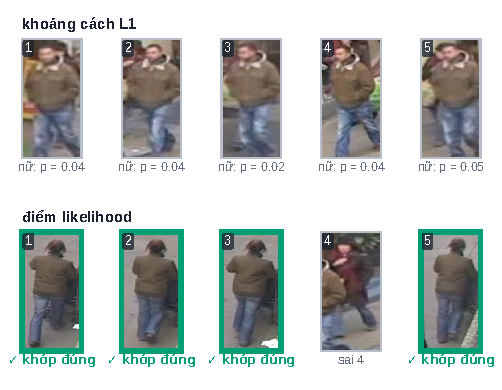
\includegraphics[width=\linewidth]{l1ll_vi.pdf}
\caption{Năm ảnh đầu của một truy vấn trên gallery PETA, dùng ensemble DINOv3 + CLIP của fold giữ ngoài PETA. Truy vấn mô tả một phụ nữ trưởng thành, tóc ngắn, mặc áo nâu và quần màu xanh lam. Hàng trên xếp theo khoảng cách L1. Năm ảnh này là một người đàn ông, chỉ khác truy vấn ở thuộc tính nữ (Gender-Female), và số dưới mỗi ảnh là xác suất nữ mà mô hình dự đoán. Hàng dưới xếp theo điểm likelihood. Khung xanh và dấu kiểm đánh dấu ảnh khớp đúng, và ``sai 4'' là số thuộc tính khác truy vấn.}
\label{fig:l1ll}
\end{figure}

Câu hỏi đầu tiên là với cùng các xác suất, cách chấm điểm ảnh ảnh hưởng tới thứ hạng nhiều đến đâu. \Cref{tab:score} so khoảng cách L1 của code mẫu với điểm likelihood trên cùng ensemble DINOv3 + CLIP. Điểm likelihood nâng mADM 7.03 điểm trên PETA và 5.61 điểm trên Market-1501, và cả năm độ đo còn lại đều tăng. Kết quả này lặp lại trên 49 mô hình của giai đoạn phát triển. Ở mọi mô hình, điểm likelihood cao hơn khoảng cách L1, với mức tăng mADM từ 3.7 đến 9.1 điểm.

\Cref{fig:l1ll} cho thấy nguyên nhân trên một truy vấn. Truy vấn mô tả một phụ nữ, nhưng khoảng cách L1 xếp năm ảnh của một người đàn ông lên đầu. Mô hình dự đoán đúng rằng người này không phải nữ, và mọi thuộc tính khác của các ảnh này khớp với truy vấn. Lỗi chắc chắn duy nhất này chỉ cộng gần 1 vào khoảng cách L1, ít hơn tổng các nghi ngờ nhỏ của các ảnh khớp đúng. Điểm likelihood phạt lỗi này nặng hơn nhiều, nên bốn ảnh khớp đúng lên năm hạng đầu. Vì điểm likelihood dùng hình dạng của cả vector xác suất, nó cũng nhạy hơn với chất lượng của các xác suất. Nhóm cũng thử thay tích các sigmoid trong mỗi nhóm thuộc tính loại trừ nhau bằng xác suất categorical $\log\mathrm{softmax}(z_G)$ của đúng giá trị truy vấn. Cách này nâng Rank-1 nhưng làm mADM giảm khoảng một điểm trên cả hai fold. Một lý do có thể là softmax chỉ giữ thứ tự giữa các giá trị trong nhóm và làm mất mức độ chắc chắn của mô hình về từng giá trị, trong khi mADM vẫn chấm điểm các ảnh gần khớp đứng trước ảnh khớp đúng.

\subsection{Group CE và kNN smoothing}
\label{sec:gce}

\begin{table}[t]
\centering
\small
\setlength{\tabcolsep}{3.5pt}
\begin{tabular}{@{}lccc@{}}
\toprule
Ensemble DINOv3 + CLIP & PETA & Market & TB \\
\midrule
Điểm likelihood & 69.84 & 74.59 & 72.22 \\
+ kNN smoothing & 70.23 & 75.31 & 72.77 \\
+ group CE & 70.89 & 75.28 & 73.08 \\
+ group CE + kNN smoothing (đã nộp) & \textbf{71.03} & 75.66 & 73.35 \\
\midrule
\quad kNN theo DINOv3 chưa fine-tune & 71.00 & 75.52 & 73.26 \\
\quad + query expansion & 70.99 & \textbf{75.94} & \textbf{73.47} \\
\bottomrule
\end{tabular}
\caption{mADM (điểm) trên held-out dataset của ensemble DINOv3 + CLIP (CLIP có điểm văn bản và WiSE-FT, seed 1), chấm bằng điểm likelihood. Group CE áp dụng cho cả hai mô hình. kNN smoothing dùng $k=50$, $\alpha=0.2$ và đặc trưng của mô hình DINOv3 đã fine-tune, trừ hàng thứ năm. TB là trung bình hai fold. Hàng thứ tư là cấu hình đã nộp, không tính student.}
\label{tab:gce}
\end{table}

Vì điểm likelihood phụ thuộc vào chất lượng của các xác suất, nhóm cải thiện chúng ngay trong lúc train bằng group CE. \Cref{tab:gce} đo group CE và kNN smoothing trên cả hai held-out dataset với cùng các mô hình. Group CE nâng mADM 1.05 điểm trên PETA và 0.69 điểm trên Market-1501. Mức tăng cũng xuất hiện ở từng mô hình đứng riêng. Ví dụ, mô hình DINOv3 tăng từ 65.95 lên 67.25 điểm trên PETA và từ 73.38 lên 74.41 điểm trên Market-1501. kNN smoothing nâng mADM 0.39 và 0.72 điểm khi dùng riêng, và thêm 0.14 và 0.38 điểm khi dùng sau group CE. Đặc trưng của DINOv3 chưa fine-tune cho mức tăng gần bằng đặc trưng đã fine-tune, nên bước làm mượt không phụ thuộc vào việc fine-tune trên đúng nhãn của bài toán. Query expansion~\cite{chum07}, cộng thêm vào điểm của mỗi ảnh độ giống của nó với ảnh đứng đầu, nâng mADM trên Market-1501 nhưng không nâng trên PETA. Cách này còn làm giảm Rank-5 và Rank-10 trên cả hai fold, nên không được dùng.

\subsection{Có sửa được sai lệch calibration sau khi train không?}
\label{sec:calib}

\begin{table}[t]
\centering
\small
\setlength{\tabcolsep}{4pt}
\begin{tabular}{@{}lcc@{}}
\toprule
 & PETA & Market \\
\midrule
NLL trên held-out dataset (nat/ảnh) & 6.20 & 5.26 \\
NLL trên dữ liệu nguồn (nat/ảnh) & 4.48 & 4.28 \\
Thành phần calibration, held-out dataset & 1.11 & 1.01 \\
Thành phần calibration, dữ liệu nguồn & 0.80 & 1.07 \\
\midrule
mADM, không hiệu chỉnh & 69.53 & 74.66 \\
mADM, hiệu chỉnh oracle & 71.95 & 76.26 \\
mADM, hiệu chỉnh khớp trên dữ liệu nguồn & 68.51 & 73.65 \\
mADM, chia logit cho $T=0.9$ & 69.16 & 74.44 \\
mADM, chia logit cho $T=1.1$ & 69.64 & 74.79 \\
mADM, chia logit cho $T=1.3$ & 69.49 & 74.82 \\
\bottomrule
\end{tabular}
\caption{Hiệu chỉnh xác suất sau khi train cho ensemble DINOv3 + CLIP (seed 1, không WiSE-FT). Hàm hiệu chỉnh là $\sigma(a_kz+b_k)$ cho từng thuộc tính. Hiệu chỉnh oracle khớp trên nhãn của held-out dataset. Dữ liệu nguồn là ảnh validation của hai dataset nguồn. Thành phần calibration là lượng NLL mà hàm hiệu chỉnh khớp trên chính các ảnh đó loại bỏ được~\cite{kull}.}
\label{tab:calib}
\end{table}

\begin{figure}[t]
\centering
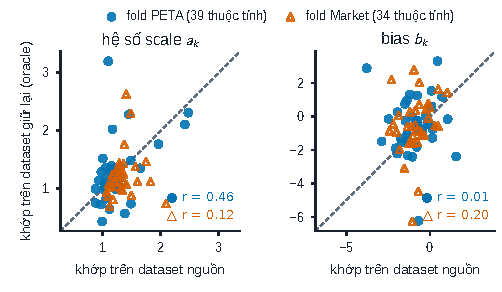
\includegraphics[width=\linewidth]{calib_vi.pdf}
\caption{Hai tham số của hàm hiệu chỉnh $\sigma(a_kz+b_k)$ cho từng thuộc tính, khớp trên dữ liệu nguồn (trục ngang) và trên nhãn của held-out dataset (trục dọc). Mỗi điểm là một thuộc tính có đủ nhãn để khớp ở cả hai nơi. Đường đứt là $y=x$, và $r$ là hệ số tương quan Pearson. Cùng ensemble như \cref{tab:calib}.}
\label{fig:calib}
\end{figure}

Ban tổ chức cho rằng mô hình trở nên quá tự tin hoặc thiếu tự tin trên camera mới~\cite{upar24}. Nhóm kiểm tra giả thuyết này bằng Platt scaling~\cite{platt} cho từng thuộc tính, $p=\sigma(a_kz+b_k)$. Hàm này được khớp theo hai cách. Cách oracle khớp trên nhãn của chính held-out dataset. Cách này không dùng được khi test, nhưng cho biết sai lệch calibration làm mất bao nhiêu điểm. Cách thứ hai khớp trên ảnh validation của hai dataset nguồn, là dữ liệu có nhãn duy nhất có sẵn khi train. Phân tích này dùng ensemble DINOv3 + CLIP với seed 1 và không có WiSE-FT, vì chỉ cấu hình này có lưu logit trên dữ liệu nguồn ở cả hai fold.

\Cref{tab:calib} cho thấy sai lệch calibration là có thật. Hiệu chỉnh oracle nâng mADM 2.42 điểm trên PETA và 1.60 điểm trên Market-1501. Tuy nhiên, hiệu chỉnh khớp trên dữ liệu nguồn làm mADM giảm khoảng một điểm trên cả hai fold. Trên 49 mô hình của giai đoạn phát triển, hiệu chỉnh này làm mADM giảm ở 48 mô hình. Ngoại lệ duy nhất là một mô hình của fold giữ ngoài PA100k, fold có tập train nhỏ hơn nhiều so với hai fold còn lại.

Nguyên nhân không phải là sai lệch calibration chỉ xuất hiện trên camera mới. Trên dữ liệu nguồn, thành phần calibration bằng 72\% thành phần trên held-out dataset ở fold PETA, và còn lớn hơn ở fold Market-1501. Lượng sai lệch giống nhau, nhưng hướng sai lệch của từng thuộc tính khác nhau (\cref{fig:calib}). Hệ số scale của phần lớn thuộc tính lớn hơn 1 ở cả hai nơi, nên mô hình hơi thiếu tự tin trên cả dữ liệu nguồn lẫn held-out dataset. Ngược lại, bias của từng thuộc tính gần như không tương quan giữa hai nơi. Một hàm khớp trên dữ liệu nguồn vì vậy dịch logit của các thuộc tính theo những hướng không khớp với camera mới. Một hệ số nhiệt độ chung cho mọi thuộc tính không có bias riêng, nhưng nó chỉ đổi mADM không quá 0.4 điểm theo cả hai chiều. Kết quả này xác nhận một phần giả thuyết của ban tổ chức. Sai lệch calibration làm mất điểm truy xuất, nhưng dữ liệu nguồn không cho biết phải sửa nó theo hướng nào. Vì vậy hệ thống của nhóm dùng xác suất thô và cải thiện chính các xác suất bằng mô hình tốt hơn.

\subsection{Vai trò của hai encoder khác nhau}
\label{sec:enc}

\begin{table}[t]
\centering
\small
\setlength{\tabcolsep}{4pt}
\begin{tabular}{@{}lccc@{}}
\toprule
Mô hình & PETA & Market & TB \\
\midrule
DINOv3 & 66.36 & 73.87 & 70.12 \\
DINOv3, trung bình hai lần train & 66.69 & 74.00 & 70.34 \\
CLIP & 65.81 & 71.72 & 68.76 \\
CLIP + điểm văn bản & 67.17 & 72.32 & 69.74 \\
CLIP + điểm văn bản + WiSE-FT & 67.38 & 71.98 & 69.68 \\
\midrule
DINOv3 + CLIP & 68.92 & 74.46 & 71.69 \\
DINOv3 + CLIP (văn bản) & 69.49 & 74.79 & 72.14 \\
DINOv3 + CLIP (văn bản, WiSE-FT) & \textbf{69.91} & \textbf{74.90} & \textbf{72.40} \\
\bottomrule
\end{tabular}
\caption{mADM (điểm) của từng mô hình và của các ensemble trên held-out dataset, chấm bằng điểm likelihood. TB là trung bình hai fold. Hàng thứ hai lấy trung bình logit của hai mô hình DINOv3, mỗi mô hình được fine-tune riêng với cùng công thức. Ensemble hai encoder khác nhau tăng nhiều hơn ensemble hai lần train của cùng một encoder. Hàng cuối là cấu hình đã nộp, không tính student.}
\label{tab:enc}
\end{table}

Vì không sửa được xác suất sau khi train, nhóm cải thiện chính các xác suất. \Cref{tab:enc} so từng mô hình với các ensemble. Lấy trung bình hai lần train của DINOv3 chỉ nâng mADM trung bình 0.22 điểm so với một lần train. Thêm CLIP vào DINOv3 nâng 1.57 điểm, dù CLIP một mình kém hơn DINOv3. Điểm văn bản và WiSE-FT của CLIP nâng ensemble thêm 0.71 điểm trung bình, phần lớn trên PETA. Student chỉ được train cho fold giữ ngoài PETA, với 10 epoch thay vì 20 epoch như student đã nộp. Thêm student này vào ensemble nâng mADM trên PETA từ 69.91 lên 70.24 điểm. Nhóm cũng thử train hai encoder trong cùng một mạng với một joint query head đọc token của cả hai, như mô hình nhóm dùng cho Track~1, với cùng loss và group CE. Mô hình này đạt 69.92 trên PETA và 75.04 trên Market-1501. Cả hai số đều thấp hơn ensemble có group CE ở \cref{tab:gce}, nên hệ thống Track~2 giữ hai encoder trong hai mô hình riêng.

\subsection{Độ nhạy của kNN smoothing}
\label{sec:knn}

\begin{table}[t]
\centering
\small
\setlength{\tabcolsep}{3.5pt}
\begin{tabular}{@{}lcccc@{}}
\toprule
Đặc trưng để tìm láng giềng & $k$, $\alpha$ & PETA & Market & PA100k \\
\midrule
không làm mượt (mADM) & & 68.45 & 78.14 & 73.86 \\
\midrule
DINOv3, TB patch token & 3, 0.25 & $-$0.03 & +0.67 & +0.52 \\
DINOv3, TB patch token & 10, 0.25 & +0.56 & +0.86 & +0.67 \\
DINOv3, TB patch token & 20, 0.25 & +0.64 & +0.86 & +0.65 \\
DINOv3, TB patch token & 50, 0.25 & +0.60 & +0.85 & +0.70 \\
DINOv3, TB patch token & 50, 0.2 & +0.70 & +0.69 & +0.66 \\
DINOv3, TB patch token & 20, 0.5 & $-$1.58 & +0.82 & $-$0.29 \\
DINOv3, token CLS & 20, 0.25 & +0.54 & +0.64 & +0.78 \\
CLIP, TB patch token & 20, 0.25 & +0.23 & +1.07 & +0.29 \\
\bottomrule
\end{tabular}
\caption{Thay đổi mADM (điểm) khi làm mượt logit theo \cref{eq:knn}, so với hàng đầu. Mô hình là ensemble DINOv3 + CLIP (không điểm văn bản) của fold giữ ngoài PETA. PETA là held-out dataset. Market và PA100k là gallery validation của hai dataset nguồn, có ảnh không dùng khi train. Hàng $k=50$, $\alpha=0.2$ là cấu hình đã nộp. TB là trung bình.}
\label{tab:knn}
\end{table}

\Cref{tab:knn} đo độ nhạy của kNN smoothing với $k$, $\alpha$ và loại đặc trưng, trên ensemble DINOv3 + CLIP của fold giữ ngoài PETA từ giai đoạn trước, với query head thường cho CLIP. Ngoài held-out dataset PETA, nhóm đánh giá trên gallery validation của Market-1501 và PA100k. Hai gallery này thuộc các dataset nguồn của fold, nhưng ảnh của chúng không được dùng khi train.

\Cref{tab:knn} cho thấy kNN smoothing theo đặc trưng của DINOv3 nâng mADM trên cả ba gallery khi $k$ từ 10 đến 50 và $\alpha$ từ 0.2 đến 0.25. Trên held-out dataset PETA, cấu hình đã nộp nâng mADM 0.70 điểm. Khi thêm student vào ensemble, mức tăng trên PETA còn 0.52 điểm. Giá trị $k$ và $\alpha$ được chọn trên chính các gallery này, nên nhóm báo cáo cả lưới tham số. Mức tăng thay đổi ít trong vùng tham số nói trên, nên nó không đến từ một điểm tham số được chọn khéo. Với $k=3$, mức tăng trên PETA biến mất. Với $\alpha=0.5$, trung bình của láng giềng có trọng số bằng dự đoán của chính ảnh, và mADM trên PETA giảm 1.58 điểm.

Phần tăng đến từ đặc trưng ngoại hình chứ không đến từ việc lấy trung bình bất kỳ. Khi láng giềng được tìm bằng cosine giữa các vector xác suất thuộc tính dự đoán, với cùng $k=50$ và $\alpha=0.2$, mADM của ensemble ở \cref{tab:score} đổi $-0.13$ điểm trên PETA và $+0.17$ điểm trên Market-1501. Với 44.6\% ảnh của PETA, láng giềng gần nhất theo đặc trưng DINOv3 có cùng cả 40 nhãn với ảnh gốc. Tỷ lệ này là 76.7\% với Market-1501 và 50.6\% với PA100k. \Cref{fig:arch}b cho thấy các láng giềng gần nhất thường là cùng một người ở các khung hình khác. Đặc trưng của DINOv3 cho mức tăng lớn hơn đặc trưng của CLIP trên PETA và PA100k, còn CLIP tốt hơn trên Market-1501.

\begin{table}[t]
\centering
\small
\setlength{\tabcolsep}{3.5pt}
\begin{tabular}{@{}lcccc@{}}
\toprule
Held-out & Mô hình & Tăng & Trung vị & Khoảng \\
\midrule
PETA & 42 & 42 & +1.08 & {[}+0.11, +1.65{]} \\
Market-1501 & 5 & 5 & +1.12 & {[}+1.00, +1.21{]} \\
\bottomrule
\end{tabular}
\caption{Thay đổi mADM (điểm) khi áp kNN smoothing ($k=50$, $\alpha=0.2$) với đặc trưng của DINOv3 ViT-H+/16 chưa fine-tune lên logit của từng mô hình của giai đoạn phát triển, chấm bằng điểm likelihood. Hai mô hình của fold giữ ngoài PA100k không có đặc trưng gallery nên không được tính.}
\label{tab:knngen}
\end{table}

Khi đặc trưng tìm láng giềng không đến từ mô hình nhận dạng, kNN smoothing trở thành một bước độc lập. Khi đó bước này áp được cho bất kỳ mô hình nào mà không cần train. \Cref{tab:knngen} áp bước này với đặc trưng của DINOv3 chưa fine-tune lên logit của 47 mô hình của giai đoạn phát triển. Mọi mô hình đều tăng mADM, với trung vị khoảng một điểm trên cả hai held-out dataset. Mức tăng nhỏ dần khi mô hình mạnh lên. Trên PETA, hệ số tương quan Pearson giữa mADM ban đầu và mức tăng là $-0.76$. Các mô hình ở đầu yếu của dải tăng khoảng 1.6 điểm, còn các mô hình ở đầu mạnh tăng từ 0.1 đến 0.9 điểm. Ensemble đã nộp nằm ở đầu mạnh của dải này, nên mức tăng của nó ở \cref{tab:gce} nhỏ hơn.

\subsection{Tập test ẩn}
\label{sec:test}

\begin{table}[t]
\centering
\small
\setlength{\tabcolsep}{4pt}
\begin{tabular}{@{}p{0.8\linewidth}c@{}}
\toprule
Bài nộp & mADM \\
\midrule
Student DINOv3 ViT-B/16 & 63.65 \\
DINOv3 + CLIP + student DINOv3 ViT-L/16 & 67.22 \\
\quad + điểm văn bản, WiSE-FT, kNN smoothing & 67.83 \\
\quad + group CE cho DINOv3 và CLIP & \textbf{68.17} \\
\bottomrule
\end{tabular}
\caption{mADM (điểm) trên tập test ẩn của UPAR 2027 Track~2. Mọi bài nộp dùng điểm likelihood. Bài nộp 67.83 có mAP 39.52, mINP 27.91, Rank-1 40.79, Rank-5 61.45 và Rank-10 69.91.}
\label{tab:test}
\end{table}

\Cref{tab:test} liệt kê bốn bài nộp có điểm được ghi lại. Bài nộp đầu là một student DINOv3 ViT-B/16 duy nhất, khi máy chấm của cuộc thi còn chạy trên CPU. Hai bài nộp sau dùng ba mô hình ở \cref{fig:arch}. Bước thứ ba thay đổi hơn một thành phần, nên không tách được đóng góp của từng thành phần, nhưng hướng thay đổi khớp với \cref{tab:enc,tab:knn}. Bước cuối chỉ thay mô hình DINOv3 và mô hình CLIP bằng bản train thêm group CE. Bước này nâng mADM 0.34 điểm, cùng chiều với \cref{tab:gce}. Leaderboard năm nay không công bố điểm của baseline trên tập test, nên nhóm không so sánh trực tiếp được với baseline.

%=====================================================================
\section{Hạn chế}
\label{sec:limits}

Các kết quả của bài được đo trên bài toán truy xuất của UPAR 2027, với ba dataset và 40 thuộc tính của cuộc thi. Nhóm chưa thử điểm likelihood, group CE và kNN smoothing trên các dataset truy xuất khác, và phân tích calibration chỉ gồm một ensemble và hai dạng hiệu chỉnh. Mức tăng của kNN smoothing phụ thuộc vào việc cùng một người xuất hiện nhiều lần trong gallery hay không, và nhóm chưa đo được điều này trên tập test ẩn. Giá trị $k$ và $\alpha$ được chọn trên chính các gallery được báo cáo, và phần lớn kết quả trên các fold chỉ có một seed. Truy xuất người theo thuộc tính trong video giám sát cũng có thể bị dùng để theo dõi một người mà không có sự đồng ý của họ, và bài này chỉ báo cáo kết quả kỹ thuật.

%=====================================================================
\section{Kết luận}
\label{sec:conclusion}

Trên camera chưa từng thấy, dự đoán của các foundation encoder đã fine-tune nên được xếp hạng bằng xác suất khớp đúng với truy vấn thay cho khoảng cách L1. Sai lệch calibration làm mất điểm truy xuất, nhưng không sửa được bằng dữ liệu của các dataset nguồn, vì hướng sai lệch của từng thuộc tính thay đổi theo domain. Thay vào đó, hai cách cải thiện chính các xác suất đều chuyển được sang dataset mới. Group CE dạy mô hình rằng mỗi nhóm thuộc tính loại trừ nhau có đúng một giá trị, còn đặc trưng ngoại hình của encoder cho phép gallery làm mượt dự đoán của chính nó. Bước tiếp theo là kiểm tra kNN smoothing trên những gallery có ít ảnh lặp lại của cùng một người.

{\small
\bibliographystyle{ieeenat_fullname}
\bibliography{refs}
}

\end{document}
